\section{Desenvolvimento}

Já desde o início de janeiro, a proposta inicial do Calopsita foi montada. Durante o mês de janeiro, estudamos tecnologias que poderiam ser interessantes no desenvolvimento do projeto e conseguimos o apoio do professor Alfredo Goldman, que aceitou nos orientar, da Caelum, que nos cedeu horas do trabalho e dos mestrandos Mariana Bravo e Hugo Corbucci, nossos clientes eleitos.

Também desde então temos o grupo de discussões~\footnote{http://groups.google.com/group/calopsita-development} e um repositório no GitHub para o projeto. Esse repositório foi movido durante o desenvolvimento, mas seu histórico completo se manteve. Abaixo, um gráfico de número de linhas enviadas ao repositório no decorrer do ano ilustra a distribuição do trabalho de código durante o ano.

\begin{figure}[htbp]
  \centering
  \fbox{
    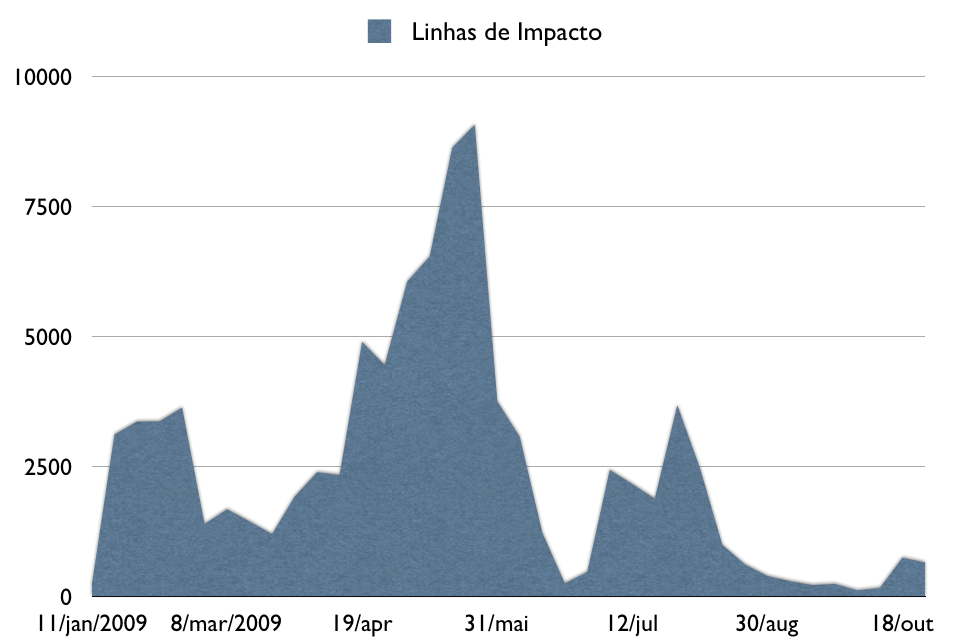
\includegraphics[width=110mm]{images/impacto.png}
  }
  \caption{Linhas de impacto - GitHub}
\end{figure}

Esses dados foram colhidos do gráfico de impacto do GitHub e as divisões de linhas por desenvolvedor foram removidas porque, como adotamos programação pareada na maioria do tempo, ele não necessariamente representa a cota de cada desenvolvedor no projeto.

Nota-se dessa imagem um pico de linhas de código enviadas ao repositório no mês de maio, mês seguinte a começarmos a gerenciar o próprio Calopsita usando a parte que já estava pronta do projeto. Contudo, houve trabalho de janeiro até o momento atual, com uma considerável queda em setembro para que focássemos nessa monografia.

\begin{figure}[htbp]
  \centering
  \fbox{
    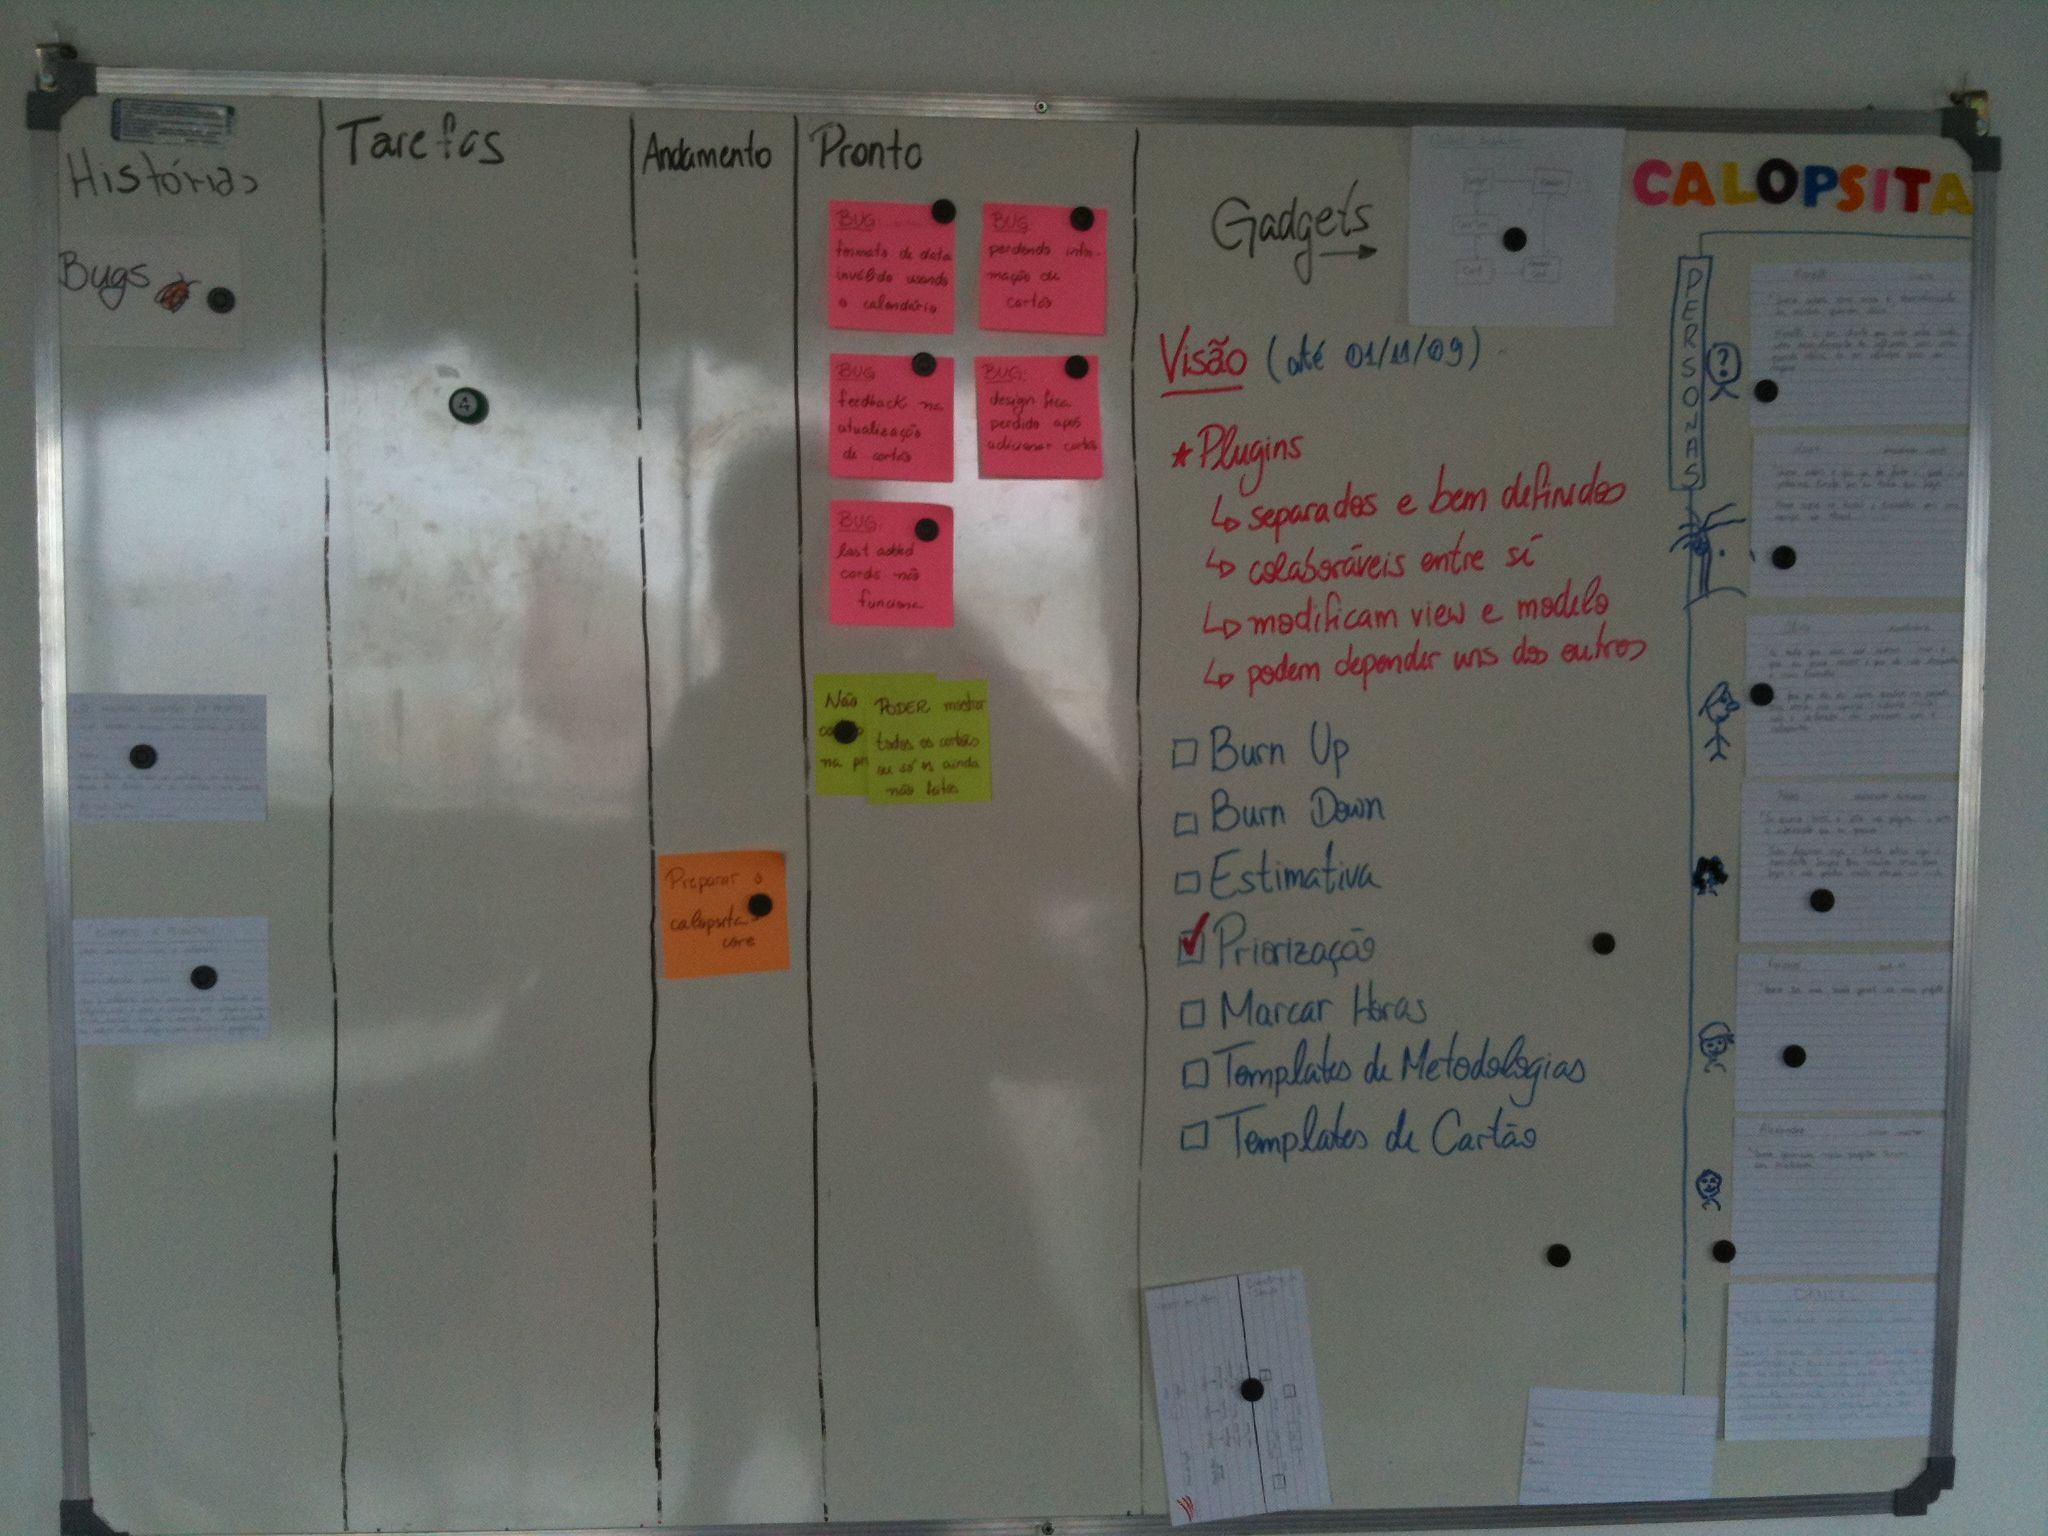
\includegraphics[width=110mm]{images/calopsita-kanban.jpg}
  }
  \caption{KanBan do Calopsita}
\end{figure}

Para mantermos a qualidade de nosso código, utilizamos desde o começo do projeto um servidor de integração contínua~\cite{ci}, o CruiseControl.rb~\footnote{http://cruisecontrolrb.thoughtworks.com/}. Esse servidor é capaz de **pingar** o repositório de código de tempos em tempos verificando por mudançar no código, e uma vez detectada alguma alteração, ele baixa o novo código, compila e roda seus testes de forma automática. Se durante esse processo, qualquer um dos testes falha, um email é disparado para toda a equipe, garantido que o bug introduzido seja corrigido o mais rapidamente possível.

\begin{figure}[htbp]
  \centering
  \fbox{
    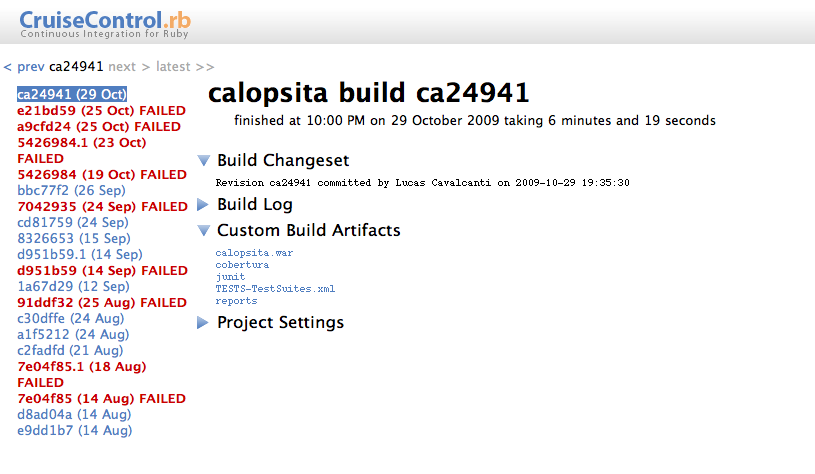
\includegraphics[width=110mm]{images/cruisecontrol-calopsita.png}
  }
  \caption{Cruisecontrol.rb do calopsita}
\end{figure}

Clientes reais e distribuidos
Muito pareamento
Kanban + Calopsita
Usamos XP e ?????
TDD e Integração Contínua

